% !TeX root = ./2021-22-COMP702-02-lecture-materials-screen.tex
% Adjust these for the path of the theme and its graphics, relative to this file
%\usepackage{beamerthemeFalmouthGamesAcademy}
\usepackage{../../beamerthemeFalmouthGamesAcademy}
\usepackage{multimedia}
\graphicspath{ {../../} }

% Default language for code listings
\lstset{language=C++,
        morekeywords={each,in,nullptr}
}

% For strikethrough effect
\usepackage[normalem]{ulem}
\usepackage{wasysym}

\usepackage{pdfpages}

% http://www.texample.net/tikz/examples/state-machine/
\usetikzlibrary{arrows,automata}

\newcommand{\modulecode}{COMP702}\newcommand{\moduletitle}{Classical Artificial Intelligence}\newcommand{\sessionnumber}{1}

\hypersetup{
pdftex,
pdftitle=\sessionnumber: Authored Behaviour,
pdfauthor=Ed Powley,
pdfdisplaydoctitle,
pdflang=en-GB
}

\begin{document}
\title{\sessionnumber: Authored Behaviour}
\subtitle{\modulecode: \moduletitle}

\frame{\titlepage} 

\part{Agents}
\frame{\partpage}

\begin{frame}{Agents}
    \begin{center}
        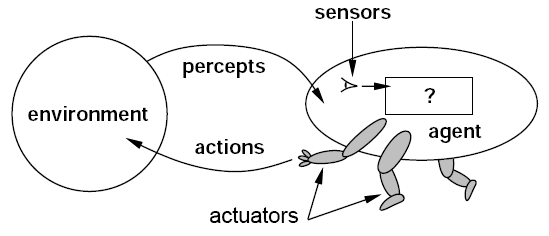
\includegraphics[width=0.7\textwidth]{agent}

        \vspace{2ex}

        \pause An \textbf{agent} is anything which perceives an \textbf{environment} through \textbf{sensors},
            and acts upon that environment through \textbf{actuators}.
    \end{center}
\end{frame}

\begin{frame}{Performance}
    \begin{itemize}
        \pause\item An ``intelligent'' agent moves towards some kind of \textbf{goal}
        \pause\item The goal is an \textbf{environment state} (or a set of states)
        \pause\item A \textbf{performance measure} evaluates a given state for how well it fits the goal
    \end{itemize}
\end{frame}

\begin{frame}{PEAS}
    For each example of an agent, what are the \underline{P}erformance measure,
        \underline{E}nvironment, \underline{A}ctuators and \underline{S}ensors?
    
    % \begin{itemize}
    %     \pause\item A Roomba
    %     \pause\item A self-driving car
    %     \pause\item A chatbot
    %     \pause\item A factory robot
    %     \pause\item An enemy in an FPS game
    %     \pause\item A chess AI
    %     \pause\item A human
    % \end{itemize}
\end{frame}

\begin{frame}{Types of environment}
    \begin{itemize}
        \pause\item Environments come with many different properties
        \pause\item These properties influence the choice of AI architecture we use to build agents
    \end{itemize}
\end{frame}

\begin{frame}{Observability}
    \begin{itemize}
        \pause\item \textbf{Fully observable}: the agent's sensors give it full information about the state of the environment
        \pause\item \textbf{Partially observable}: some aspects of the environment state are not visible to the agent's sensors
        \pause\item E.g.\ a chess game is fully observable, a poker game is partially observable
    \end{itemize}
\end{frame}

\begin{frame}{Number of agents}
    \begin{itemize}
        \pause\item \textbf{Single agent}: our agent is the only one in the environment
        \pause\item \textbf{Multi-agent}: there is more than one agent
        \pause\item \textbf{Cooperative}: all agents share the same performance measure
        \pause\item \textbf{Competitive}: agents' performance measures are in opposition to each other
            (i.e.\ if one agent ``wins'', another ``loses'')
    \end{itemize}
\end{frame}

\begin{frame}{Determinism}
    \begin{itemize}
        \pause\item \textbf{Deterministic}: the next state of the environment is completely determined by the current state and by the agent's action
        \pause\item \textbf{Stochastic}: there is some aspect of randomness in determining the next state
        \pause\item E.g.\ chess is deterministic; any board game involving dice rolls or random card draws is stochastic
    \end{itemize}
\end{frame}

\begin{frame}{Dynamicity}
    \begin{itemize}
        \pause\item \textbf{Static}: the environment does not change while the agent is deliberating
        \pause\item \textbf{Dynamic}: the environment changes constantly
        \pause\item E.g.\ most board games are static, most (non turn-based) video games are dynamic
    \end{itemize}
\end{frame}

\begin{frame}{Discreteness}
    \begin{itemize}
        \pause\item \textbf{Discrete}: time, percepts and actions are all discrete
            (from a finite set of possibilities or ``integer valued'')
        \pause\item \textbf{Continuous}: at least one of these is not discrete
            (``float valued'')
        \pause\item Continuous problems are hard so we sometimes \textbf{discretise} them
    \end{itemize}
\end{frame}

\begin{frame}{Known or unknown}
    \begin{itemize}
        \pause\item Are all the details of the environment \textbf{known} to the AI designer?
        \pause\item For a game or simulation: probably \textbf{yes}
            (unless someone else made it and we don't have the source code)
        \pause\item For the real world: technically \textbf{no}
            (but we have physics, sociology, economics etc to give us good approximations)
    \end{itemize}
\end{frame}

\begin{frame}{Agents and AI}
    \begin{itemize}
        \pause\item The ideas of agents and environments are a useful frame for designing AI
        \pause\item All(?) AI problems can be expressed in terms of creating an agent
            that optimises some performance measure in some environment
        \pause\item Agent design boils down to: given a \textbf{percept} (and possibly some \textbf{memory} of past percepts/actions),
            choose the best \textbf{action} to take now
    \end{itemize}
\end{frame}

\part{Rule-based AI}
\frame{\partpage}

\begin{frame}{Rule-based AI}
	\begin{itemize}
		\pause\item Generally \textbf{reactive} to the state of the world
		\pause\item Based on \textbf{if-then} triggers, basic \textbf{calculations}, etc.
		\pause\item Generally hand-coded and only modifiable by a programmer
	\end{itemize}
\end{frame}

\begin{frame}{Case study: Ghosts in Pac-Man}
	\begin{itemize}
		\pause\item Full details: \url{http://gameinternals.com/understanding-pac-man-ghost-behavior}
		\pause\item Each ghost has 3 states
			\begin{itemize}
				\pause\item Chase: head for a specific position (see next slide)
				\pause\item Scatter: head for a specific corner of the level
				\pause\item Frightened: move randomly
			\end{itemize}
	\end{itemize}
\end{frame}

\begin{frame}{Ghost ``personalities''}
	\begin{itemize}
		\pause\item Red ghost: aim for Pac-Man
		\pause\item Pink ghost: aim for 2 spaces ahead of Pac-Man
		\pause\item Blue ghost: aim for position on the line between red ghost and 2 spaces ahead of Pac-Man
		\pause\item Orange ghost: aim for Pac-Man until 8 spaces away, then aim for corner
	\end{itemize}
\end{frame}

\begin{frame}{Ghost movement}
	\begin{itemize}
		\pause\item No pathfinding --- greedily move towards target
		\pause\item Can only change direction at an intersection
		\pause\item Can't reverse or stay still
		\pause\item Therefore can't get stuck, despite imperfect pathfinding
	\end{itemize}
\end{frame}

\begin{frame}{Ghost behaviour}
	\begin{itemize}
		\pause\item Behaviour rules are very simple
		\pause\item However, the combination of them leads to interesting gameplay and illusion of personality
	\end{itemize}
\end{frame}

\begin{frame}{Design lessons}
	\begin{itemize}
		\pause\item AI doesn't have to be complicated
		\pause\item Simple AI, when interacting with a player and each other, can give engaging results
		\pause\item Bugs in AI don't always matter...
	\end{itemize}
\end{frame}


\part{Finite state machines}
\frame{\partpage}

\begin{frame}{Finite state machines}
    \begin{itemize}
        \item A \textbf{finite state machine (FSM)} consists of: \pause
            \begin{itemize}
                \item A set of \textbf{states}; and \pause
                \item \textbf{Transitions} between states \pause
            \end{itemize}
        \item At any given time, the FSM is in a \textbf{single state} \pause
        \item \textbf{Inputs} or \textbf{events} can cause the FSM to transition to a different state
    \end{itemize}
\end{frame}

\begin{frame}{State transition diagrams}
    \begin{center}\scalebox{0.8}{
        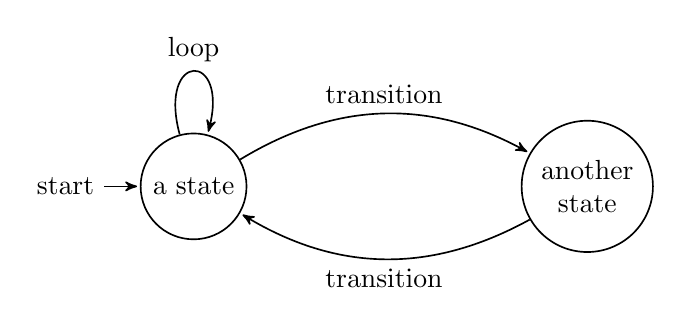
\begin{tikzpicture}[->,>=stealth',shorten >=1pt,auto,node distance=5cm,
                            semithick]
            \node[initial,state] (A) {a state};
            \node[state] (B) [right of=A, align=center] {another\\state};

            \path (A) edge [bend left] node [above] {transition} (B)
                  (B) edge [bend left] node [below] {transition} (A)
                  (A) edge [loop above] node {loop} (A);
        \end{tikzpicture}
    }\end{center}
    \begin{itemize}
        \pause\item FSMs are often drawn as \textbf{state transition diagrams}
        \pause\item Reminiscent of \textbf{flowcharts} and certain types of \textbf{UML diagram} 
    \end{itemize}
\end{frame}

\begin{frame}{FSMs for AI behaviour}
    The next slide shows a simple FSM for the following AI behaviour, for an enemy NPC in a shooter game: \pause
    \begin{itemize}
        \item By default, patrol (e.g.\ along a preset route) \pause
        \item If the player is spotted, attack them \pause
        \item If the player is no longer visible, resume patrolling \pause
        \item If you are low on health, run away and find a medikit. Then resume patrolling \pause
        \item If you are low on ammo, run away and find ammo. Then resume patrolling 
    \end{itemize}
\end{frame}

\begin{frame}
    \begin{center}\scalebox{0.8}{
        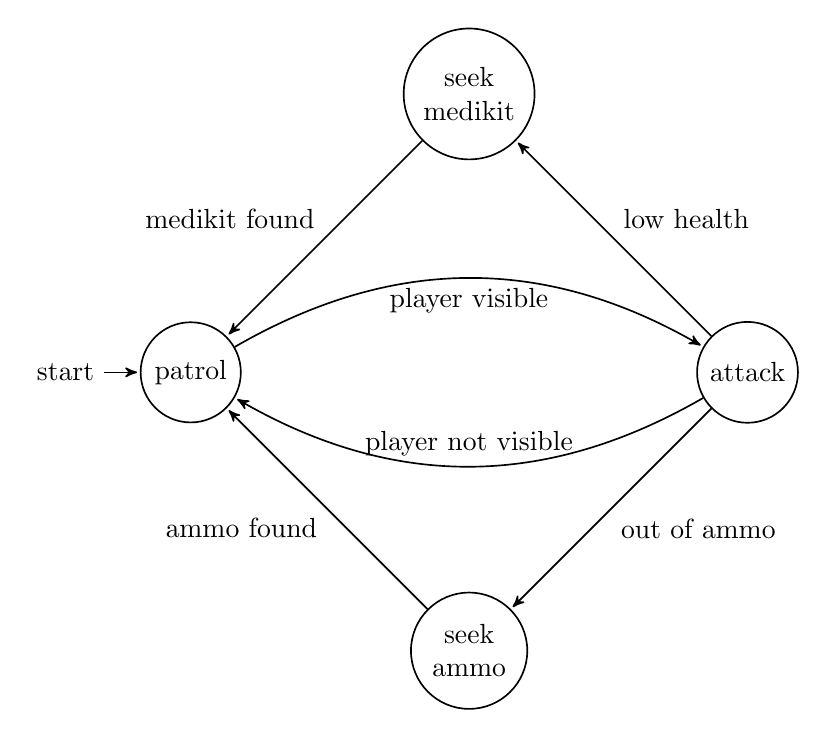
\begin{tikzpicture}[->,>=stealth',shorten >=1pt,auto,node distance=5cm,
                            semithick]
            \node[initial,state] (patrol) {patrol};
            \node[state] (health) [above right of=patrol, align=center] {seek\\medikit};
            \node[state] (ammo) [below right of=patrol, align=center] {seek\\ammo};
            \node[state] (attack) [above right of=ammo] {attack};

            \path (patrol) edge [bend left] node [below] {player visible} (attack)
                  (attack) edge [bend left] node [above] {player not visible} (patrol)
                  (attack) edge node [above right] {low health} (health)
                  (attack) edge node {out of ammo} (ammo)
                  (health) edge node [above left] {medikit found} (patrol)
                  (ammo) edge node {ammo found} (patrol);
        \end{tikzpicture}
    }\end{center}
\end{frame}

\begin{frame}{Other uses of FSMs}
    As well as AI behaviours, FSMs may also be used for: \pause
    \begin{itemize}
        \item Animation \pause
        \item UI menu systems \pause
        \item Dialogue trees \pause
        \item Token parsing \pause
        \item ...
    \end{itemize}
\end{frame}

\begin{frame}{Beyond FSMs}
    Some topics for you to research, for when plain old FSMs aren't enough... \pause
    \begin{itemize}
        \item Hierarchical FSMs
        \item Nested FSMs
        \item Stack-based FSMs
        \item Hierarchical task networks
        \item ...
    \end{itemize}
\end{frame}

\part{Behaviour Trees}
\frame{\partpage}

\begin{frame}{Behaviour trees (BTs)}
	\begin{itemize}
		\pause\item A \textbf{hierarchical} model of decision making
		\pause\item Allow \textbf{complex behaviours} to be built up from \textbf{simple components}
		\pause\item Allow for \textbf{more complex} behaviours than FSMs
		\pause\item First used in Halo 2 (2005), now used extensively
		\pause\item Also used in robotics and other non-game AI applications
	\end{itemize}
\end{frame}

\begin{frame}{Using BTs}
	\begin{itemize}
		\pause\item Fairly easy to implement; plenty of resources online
		\pause\item \textbf{Unreal}: an advanced BT system is built in
		\pause\item \textbf{Unity}: numerous free and paid options on the Asset Store
			e.g.\ Behavior Machine, Behavior Designer, Behave, RAIN
	\end{itemize}
\end{frame}

\begin{frame}{BT basics}
	\begin{itemize}
		\pause\item A BT is a \textbf{tree} of \textbf{nodes}
		\pause\item On each game update (i.e.\ each frame), the root node is \textbf{ticked}
			\begin{itemize}
				\pause\item When a node is ticked, it might cause some or all of its \textbf{children} to tick as well
				\pause\item So ticks propagate down the tree from the root
			\end{itemize}
		\pause\item A ticked node returns one of three \textbf{statuses}:
			\begin{itemize}
				\pause\item Success
				\pause\item Running
				\pause\item Failure
			\end{itemize}
		\pause\item ``Running'' status allows nodes to represent operations that \textbf{last multiple frames}
	\end{itemize}
\end{frame}

\begin{frame}{Blackboard}
	\begin{itemize}
		\pause\item It is often useful to \textbf{share} data between nodes
		\pause\item A \textbf{blackboard} (sometimes called a \textbf{data context}) allows this
		\pause\item Blackboard defines \textbf{variables}, which can be \textbf{read} and \textbf{written} by nodes
		\pause\item Blackboard can be \textbf{local} to the AI agent, \textbf{shared} between several agents, or \textbf{global} to all agents
		\pause\item (Shared blackboards mean that your AI has ``telepathy'' --- this may or may not be desirable!)
	\end{itemize}
\end{frame}

\begin{frame}{BTs in The Division}
	\begin{center}
		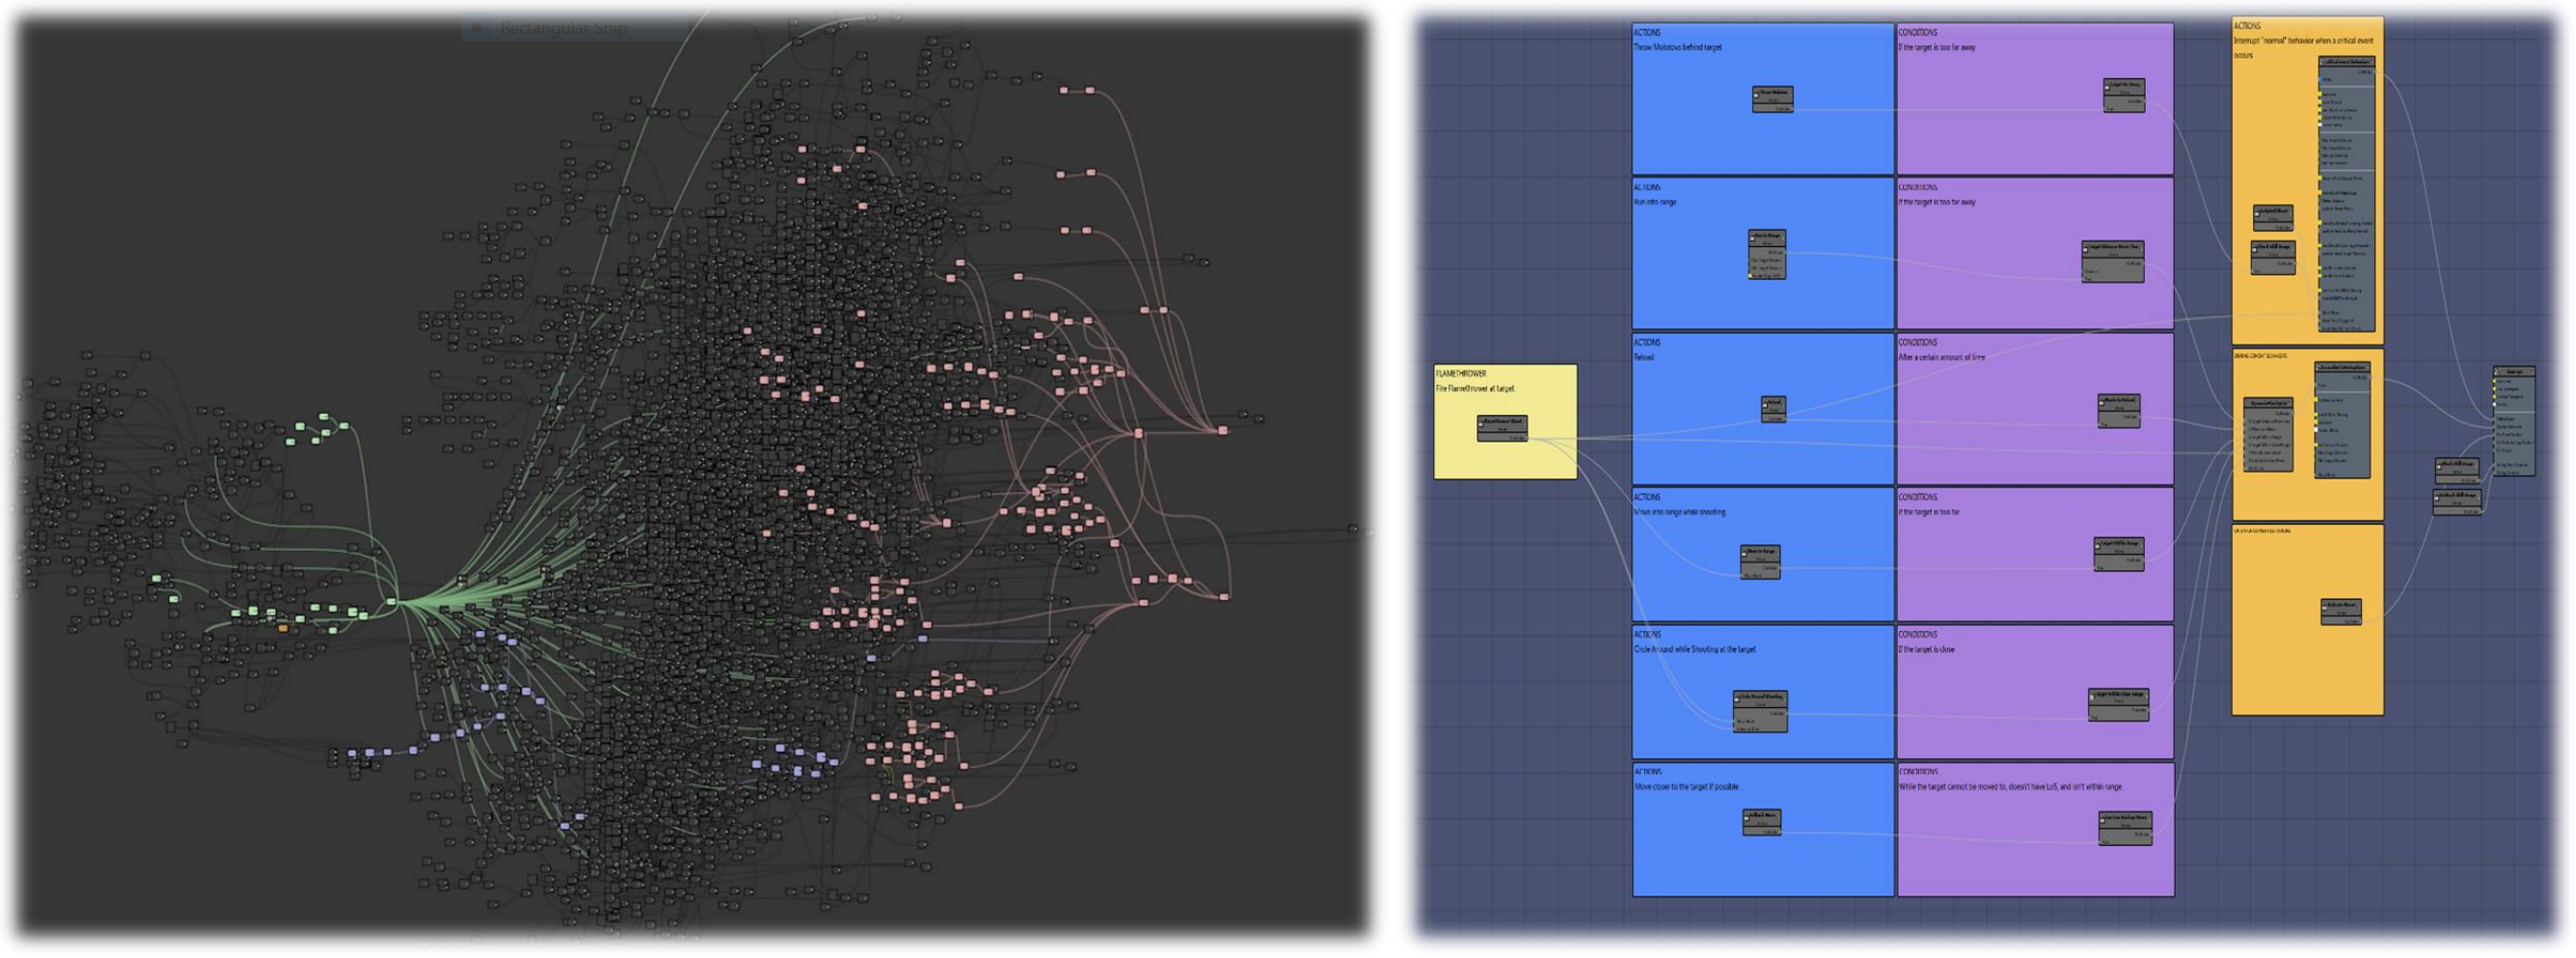
\includegraphics[width=\textwidth]{the_division}
		
		\url{http://www.gdcvault.com/play/1023382/AI-Behavior-Editing-and-Debugging}
	\end{center}
\end{frame}

 
\part{Workshop}
\frame{\partpage}

\end{document}
